\chapter{Experimental Framework}

\MyQuote{What we observe is not nature itself, but nature exposed to our method of
questioning.}{Werner Heisenberg}

In the previous chapter, the key features of QCD - today's theory of strong
interaction - were introduced. The predictions of QCD are tested at particle
accelerators persistently with no signs for new physics so far. Large Hadron
Collider which will open energy regions not observed yet can change this very
soon.

Jets are the most important objects observed by inelastic collisions on hadron
colliders, which allows the QCD predictions to be confronted with the
experiment. In this chapter, after the introduction of the Large Hadron Collider
and the ATLAS detector, jet algorithms and the way how jets are reconstructed on
the ATLAS detector will be described.

\section{The Large Hadron Collider and The ATLAS Detector}

\subsection{The Large Hadron Collider}

The Large Hadron Collider (LHC) \cite{LHC, LHCPastPresentFuture} is a charged
particle accelerator located on the border of France and Switzerland, near
Geneva at CERN (the European Organization for Nuclear Research) in Switzerland.
Built using the areas of the Large Electron-Positron collider, the main
accelerator ring, of a 27 km circumference, is located around 100 m below the
surface. There are four main experiments located around the ring: A Large Ion
Collider Experiment (ALICE), A Toroidal LHC ApparatuS (ATLAS), Compact Muon
Solenoid (CMS) and Large Hadron Collider beauty (LHCb). The complete accelerator
and detector system is shown in Figure \ref{fig:LHC}.

\begin{figure}[t]
  \centering
  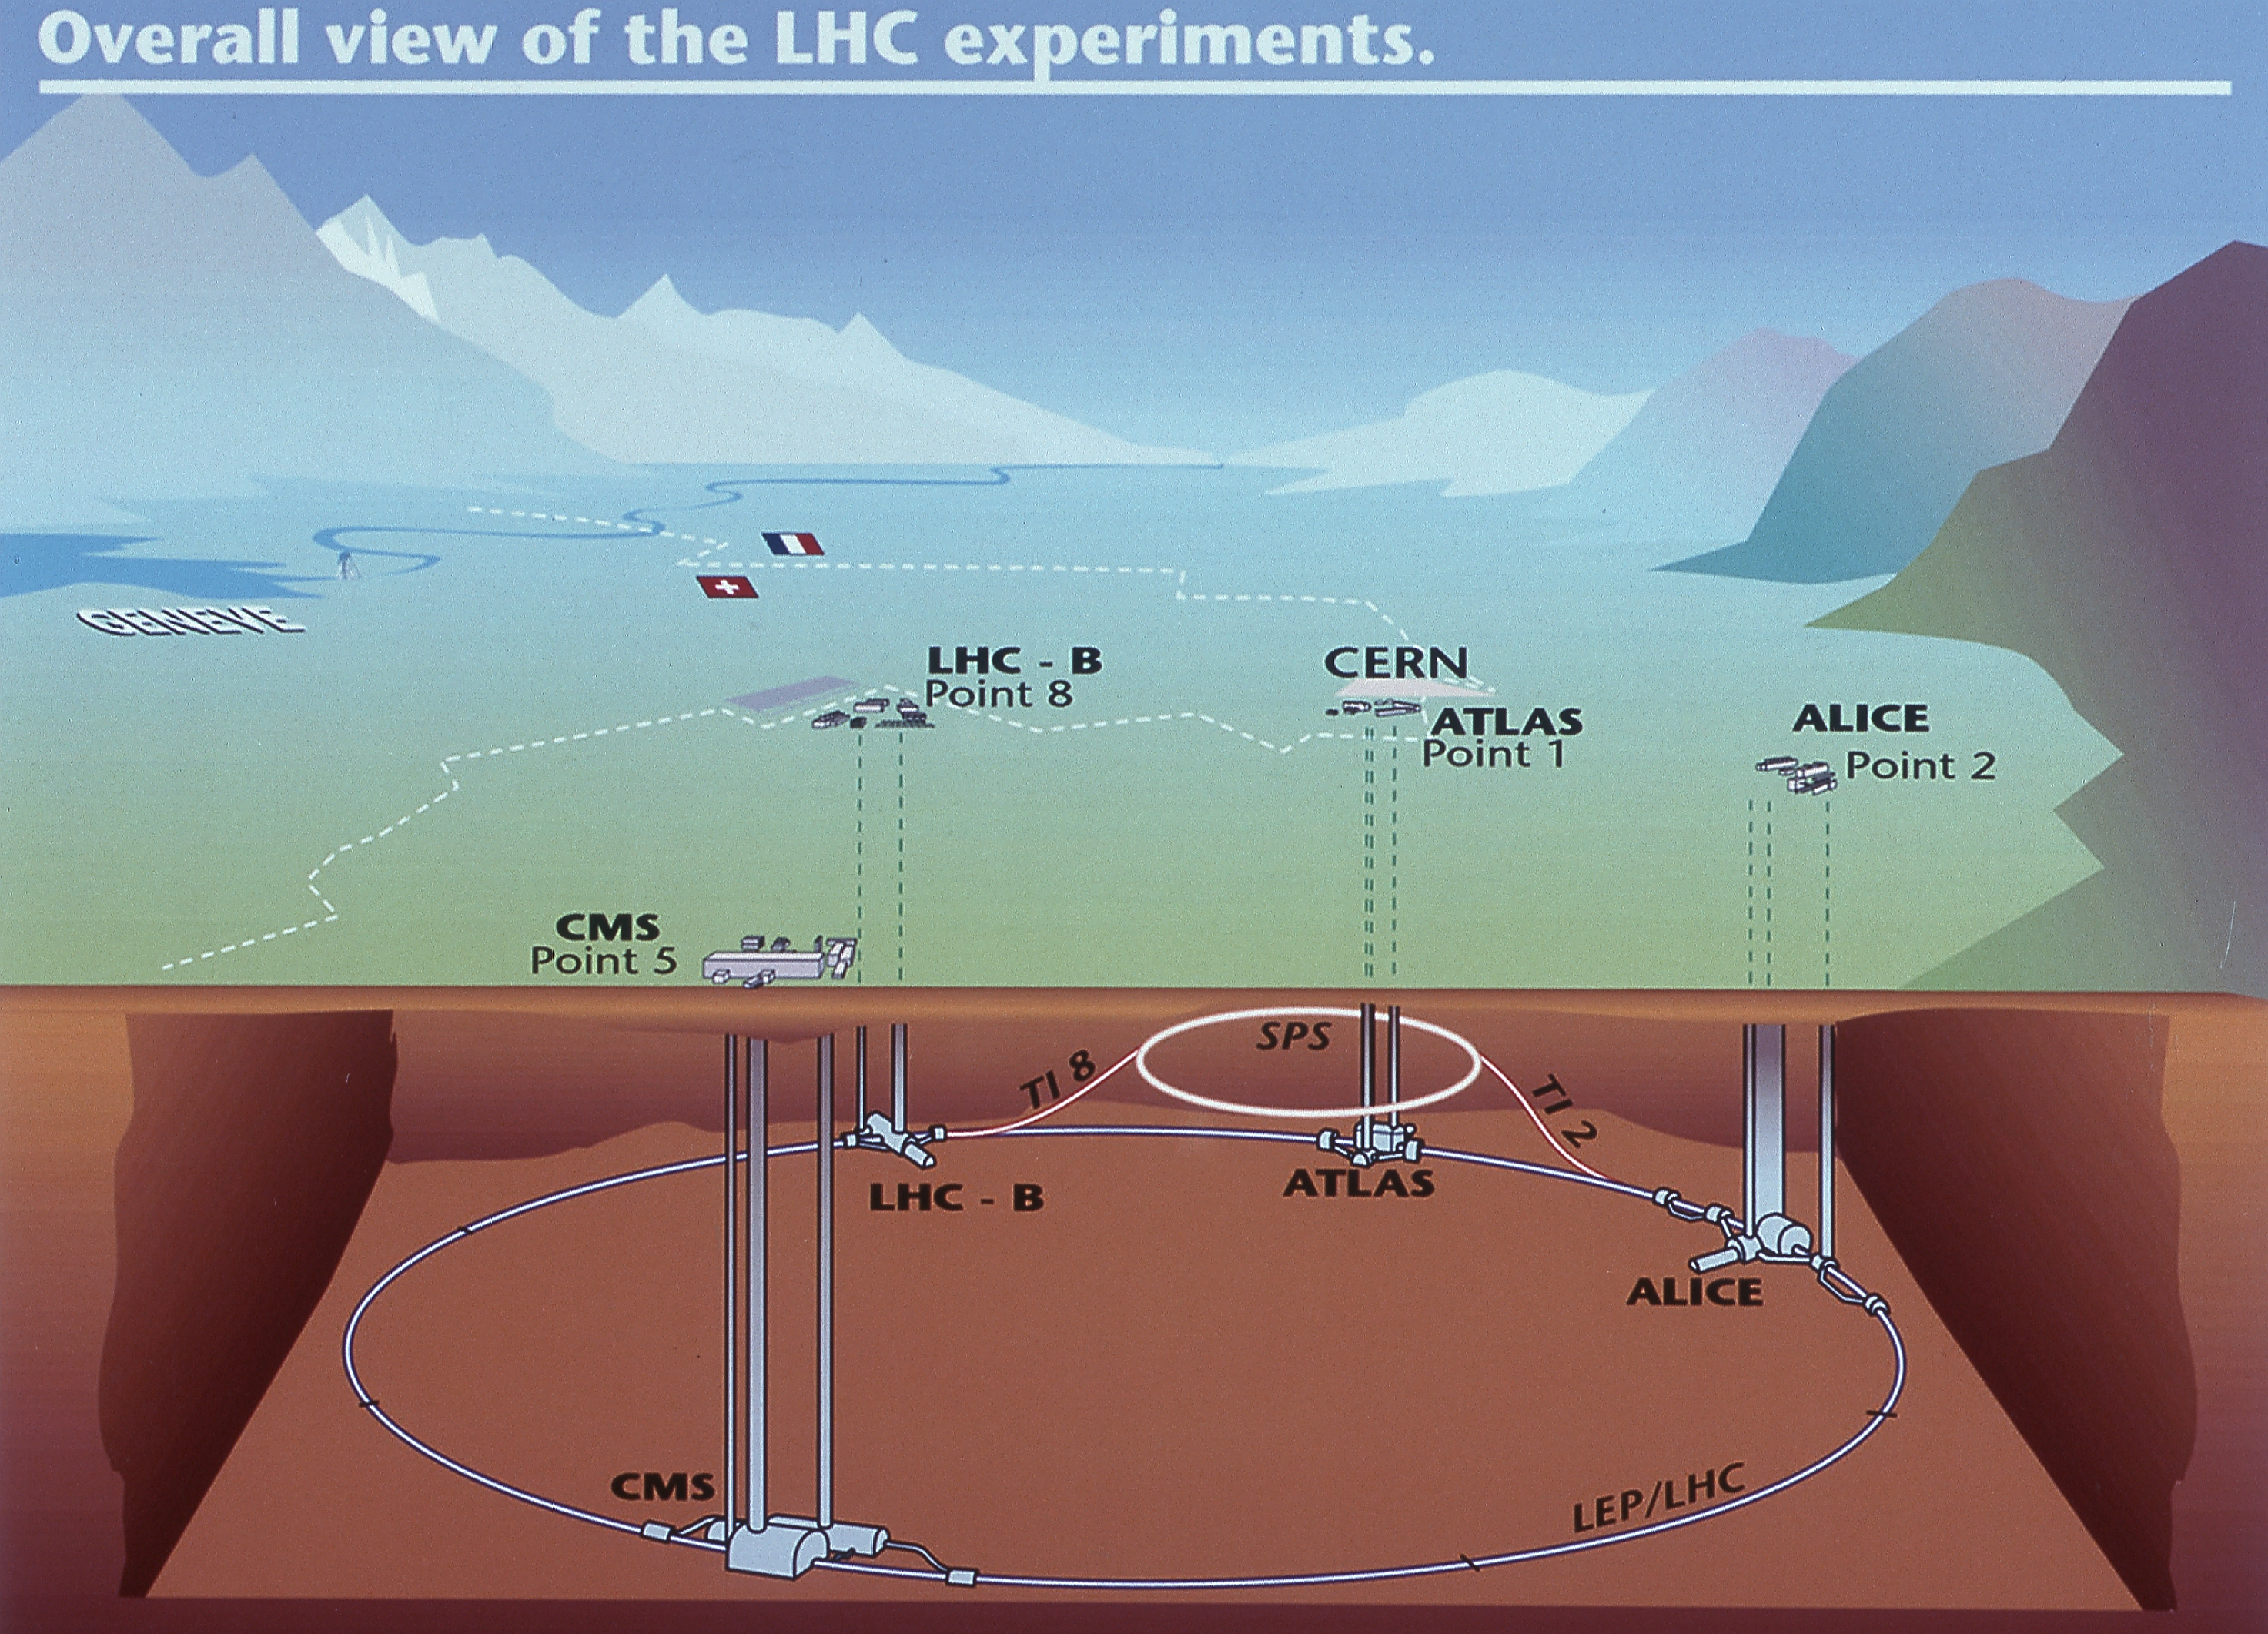
\includegraphics[width=0.8\textwidth]{Chapter2/LHC.jpg}
  \caption{This diagram shows the locations of the four main experiments (ALICE,
    ATLAS, CMS and LHCb) that take place at the LHC. Located between 50 m and
    150 m underground, huge caverns have been excavated to house the giant
    detectors. The Super Proton Synchotron (SPS), the final link in the
    pre-acceleration chain, and its connection tunnels to the LHC are also
    shown.  Figure from \cite{CERN:ATLASexperimentPictureswiki}.  }
  \label{fig:LHC}
\end{figure}

LHC started to operate on November 23, 2009 and soon thereafter (March 30, 2010)
the proton-proton collisions achieved the center-of-mass energy $\sqrt{s} = 7
\TeV$, which is a half of the design energy of the machine. On April 5, 2012, the
machine started its successful $\sqrt{s} = 8 \TeV$ run.

Next to the proton-proton collisions, first heavy-ion Pb-Pb collisions took place
in 2010 at a center of mass energy per pair of colliding nucleons $\sqrt{s} =
2.76 \TeV$. Proton-Pb collisions at $\sqrt{s} = 5.02 \TeV$ occurring on LHC
during 3 weeks of 2013 successfully demonstrated LHC capability to provide
asymmetric collisions.  

The first running period of the LHC, Run I, was very successful and resulted in
the discovery of the Higgs boson on July 4, 2012 \cite{HiggsDiscovery}.  The
accelerator complex including its experiments has been upgraded for two years
and the Run II is expected to start in early summer 2015 \cite{LHCFuture,
LHCFutureLuminosigy}. In Run II the center-of-mass energy of proton-proton
collisions will be raised to $\sqrt{s} = 13 \TeV$ and the beam crossing time
could be reduced from the current $50\,\text{ns}$ to $25\,\text{ns}$. The
expected integrated luminosity is expected to be $\sim 100\,\text{fb}^{-1}$
after three years of data collecting.

\subsection{The ATLAS Detector}

The ATLAS detector \cite{ATLAS} is a general-purpose detector surrounding one of
the interaction points of the LHC and with $\sim 100$ million of individual
electronic channels it is the most complicated instrument ever created.
The purpose of the ATLAS detector is to record particle collisions up to the center-of-mass
energy per pair of colliding nucleons $\rts = 14 \TeV$. A detector overview is
shown in Figure~\ref{fig:ATLASfull}, where the main sub-detector systems can be
seen: the inner detector, used to reconstruct charged-particle tracks, the
electromagnetic calorimeters, the hadronic calorimeters, and the muon
spectrometer. 

\begin{figure}[p]
  \centering
  \begin{subfigure}[b]{0.9\textwidth}
    \includegraphics[width=\textwidth]{Chapter2/ATLAS.png}
    \caption{ATLAS detector.}
    \label{fig:ATLASfull}
  \end{subfigure}
  ~
  \begin{subfigure}[b]{0.9\textwidth}
    \includegraphics[width=\textwidth]{Chapter2/ATLASinner.jpeg}
    \caption{Inner detector and calorimeter systems.}
    \label{fig:ATLASinner}
  \end{subfigure}
  \caption{(a) an overview of the ATLAS detector 
           (b) detail on the inner detector and the calorimeters - the dominant
           sub-detector systems used in this thesis. Figures taken from
           \cite{CERNbook}.}
  \label{fig:ATLAS}
\end{figure}

ATLAS uses a right-handed coordinate system with its origin at the interaction
point in the center of the detector and the $z$ axis along the beam pipe. The
$x$ axis points from the interaction point to the center of the LHC ring, and
the $y$ axis points upward. Cylindrical coordinates $(r, \phi)$ are used in the
transverse plane, $\phi$ being the azimuthal angle around the beam pipe. Instead
of polar angle $\theta$, pseudorapidity $\eta$ is often used. In this thesis
the rapidity $y$ is used as the polar angle coordinate. In following
definitions of pseudorapidity $\eta$ and rapidity $y$, $E$ stands for the total
energy and $p$ for size of total momentum: 
\begin{eqnarray}
  \eta &= & - \frac{1}{2} \ln \left( \frac{p+p_z}{p-p_z} \right) = - \ln \left[
  \tan \left( \frac{\theta}{2} \right) \right], \\ y &= &- \frac{1}{2} \ln
  \left( \frac{E+p_z}{E-p_z} \right).	
\end{eqnarray}
The transverse momentum $\pt = \sqrt{p_x^2 + p_y^2}$ presents the component of
momentum perpendicular to the beam line.  

The main detector system relevant to this thesis is the ATLAS calorimeter,
which is emphasized in Figure~\ref{fig:ATLASinner}. The calorimeter is divided
into sub-detectors, providing overall coverage up to $|\eta| < 4.9$. The
electromagnetic calorimeter, covering region $|\eta| < 3.2$, is a
high-granularity sampling detector in which the liquid argon (LAr) active medium
is interspaced with layers of lead absorber. The hadronic calorimeters are
divided into three sections: a tile scintillator/steel calorimeter is used in
both the barrel ($|\eta| < 1.0$) and extended barrel cylinders ($0.8 < |\eta| <
1.7$) while the hadronic endcap ($1.5 < |\eta| < 3.2$) consists of LAr/copper
calorimeter modules. The forward calorimeter measures both electromagnetic and
hadronic energy in the range $3.2 < |\eta| < 4.9$ using LAr/copper and
LAr/tungsten modules. 

\section{Hadron Collision at LHC}

In this section the phenomenological description of proton-proton collisions
will be presented following Figure \ref{fig:HardProcess} and
Reference about Monte Carlo event generators \cite{PDG}.

\begin{figure}[t]
  \centering
  \includegraphics[width=0.7\textwidth]{Chapter2/HardProcess.png}
  \caption{Schematic representation of a hard scattering proton-proton
    collision. Figure taken from \cite{HardProcess}.}
  \label{fig:HardProcess}
\end{figure}

Two incoming protons can be understood as two bags of partons. The collision is
dominated by the strong interaction of two partons - one from each of the
colliding hadrons. These partons are called incoming partons and the
momentum transfer of their interaction is $Q \gg \Lambda$, so the perturbative
QCD can be used to describe the process of hard scattering. The remaining energy
is carried by the remaining partons, which create the so called underlying event -
particles, which do not come from the hard QCD processes.

When partons are sufficiently far from each other, the non-perturbative QCD has to
be used to describe the process of hadronisation, in which a set of colored
partons is transformed into a set of colorless primary hadrons which may then
decay further. 

During the collision, the color charges of partons interact resulting in
radiation of gluons $q \rightarrow qg$. This process is described by
perturbative QCD and leads to infrared and collinear divergences. However,
infrared divergences are
canceled by Kinoshita--Lee--Nauenberg theorem \cite{KLN1,KLN2}, so only
collinear divergences remain. There is no mechanism known up to date, which
would solve the problem with collinear divergences. However, observables
inclusive enough to be insensitive to processes that distinguish between
different numbers of partons are not affected by infrared divergences.
There is no possibility how to theoretically predict the energy of hardest
outgoing particle, but it is possible to predict the energy flow in a cone from
the point of scattering.

This is where the term jet comes to play. A jet can be naively seen as a group
of collimated particles generated by the hadronisation of a parton in the
scattering process and is the most important object used on hadron colliders for
analysis of QCD processes.

\section{Jet Algorithms}

Jet algorithm is a generic "recipe" which takes a set of particles (or other
objects with defined four-momenta) and returns jets created from them. The jet
algorithm usually involves a set of parameters which togetger with the algorithm fully specify
the jet definition. According to the remarks at the end of the previous section,
jet algorithms should fulfill the following conditions 

\begin{enumerate}
  \item Infrared safety - the presence of additional soft particles should not
    affect the recombination of these particles into a jet.
  \item Collinear safety - jet reconstruction should not depend on the fact, if
    the transverse momentum is carried by one particle, or if the particle is split
    into two collinear particles.
\end{enumerate}
Two important steps must be defined in each jet algorithm

\begin{enumerate}
  \item Clustering - description how the input objects are clustered into jets.
  \item Recombination - determination of physical quantities of jets.
\end{enumerate}
Additional steps may include the preclustering reducing the number of input
objects for jet algorithm.

Two classes of jet algorithms are described here - cone algorithms and $k_t$
algorithms. First of these algorithms is more illustrative, the second one is
used in ATLAS. These algorithms use two different recombination schemes which
description will follow.  Detailed description as well as other jet algorithms
can be found in \cite{ATLASmain,JetDoporuceniZdenek}. After the definition of jet
algorithms a short description follows, how the objects (not necessary particles)
with defined four-momenta are constructed from the signal observed on the ATLAS
detector.

\subsection{Cone algorithms}

The first step of these algorithms is to order all input objects (reconstructed
detector objects with four-momentum representation) in decreasing order of
transverse momentum $\pt$. If the object with the highest $\pt$ is above the
seed threshold, all objects within a cone in rapidity $y$ and azimuth
$\phi$ with $\Delta R = \sqrt{\Delta y^2 + \Delta \phi^2} < R_{cone}$, where
$R_{cone}$ is the fixed cone radius, are recombined using Snowmass recombination
scheme (see Section \ref{sse:Recombination}).  A new cone is centered around a
new direction and the objects in the new cone are recombined and again the
direction is updated. This process continues until the direction of the cone
does not change anymore after recombination, at which point the cone is
considered stable and is called a proto-jet. 

At this point, the next seed is taken from the input list and a new proto-jet is
formed with the same iterative procedure. This continues until no more seeds are
available. 

The proto-jets found by this procedure can share some constituents. Constituents
shared between two proto-jets are recombined into new proto-jet and if the ratio
$E_T^{shared} / \text{min} ( E_T^{neighbor} ) > f$ is over the certain threshold
for example 
$f = 0.5$ the neighboring proto-jets are recombined into one proto-jet (shared
constituents are taken only once). If this condition is not satisfied, the
shared constituents are assigned to the nearest proto-jet. When proto-jet does
not share constituents it is recombined into the jet.

This algorithm is both not infrared safe (Figure \ref{fig:IRsafety}) and not
collinear safe (Figure \ref{fig:ColSafety}). The infrared insensitivity can be
improved by adding the midpoints between pairs of proto-jets fulfilling
$R_{cone} < \Delta R < 2 R_{cone}$ and repeating the iterative procedure with
midpoints being new seeds. Since the collinear unsafety arises from the use of
seed towers, Seedless cone algorithm was developed, which searches the entire
detector to find all stable proto-jets.

\begin{figure}[t]
  \centering
  \begin{subfigure}[b]{0.65\textwidth}
    \includegraphics[width=\textwidth]{Chapter2/IRsafety.png}
    \caption{Infrared unsafety}
    \label{fig:IRsafety}
  \end{subfigure}
  ~
  \begin{subfigure}[b]{0.6\textwidth}
    \includegraphics[width=\textwidth]{Chapter2/ColSafety.png}
    \caption{Collinear unsafety}
    \label{fig:ColSafety}
  \end{subfigure}
  \caption{Illustration of (a) infrared unsafety and (b) collinear unsafety
    of fixed cone jet algorithm.
    Figures from \cite{JetTheoreticalPictures}.}
  \label{fig:JetIRCOLsafety}
\end{figure}

Typical parameters used by fixed cone algorithm are a seed threshold of $\pt > 1 \GeV$,
and a narrow ($R_{cone} = 0.4$) or a wide cone jet ($R_{cone} = 0.7$) option.

\subsection{$k_t$ algorithms}

In this class of algorithms all pairs $(i,j)$ of input objects are analyzed with
respect to their relative transverse momentum squared, defined by 

\begin{equation}
	d_{ij} = \min{\left( p_{T,i}^{2p} , p_{T,j}^{2p} \right)} \frac{\Delta R_{ij}^2}{R^2}
\end{equation}
and the squared $\pt$ of object $i$ relative to the beam axis

\begin{equation}
	d_i = p_{T,i}^{2p}.
\end{equation}
Here $\Delta R_{ij}^2 = (y_i - y_j)^2 + (\phi_i - \phi_j)^2$ and $p_{T,i}$,
$y_i$ and $\phi_i$ are respectively the transverse momentum, rapidity and
azimuth of particle $i$. In addition to the radius parameter $R$, parameter $p$
was added to split $k_t$~algorithms into three categories.  
\begin{itemize}
	\item $p = 1$ $k_t$ algorithm,
	\item $p = 0$ Cambridge/Aachen algorithm,
	\item $p = -1$ anti-$k_t$ jet-clustering algorithm.
\end{itemize}

These algorithms first find the minimum $d_{min}$ of all $d_{ij}$ and $d_i$. If
$d_{min}$ is in $d_{ij}$'s, the corresponding objects $i$ and $j$ are combined
into a new object $k$ using four-momentum recombination. Both objects $i$ and
$j$ are removed from the list, and the new object $k$ is added to it. If
$d_{min}$ is in $d_i$'s, the object $i$ is considered to be a jet by itself and
is removed from the list.

This means that all original input objects end up to be either part of a jet or
to be jets by themselves. Contrary to the cone algorithm described earlier, no
objects are shared between jets and the procedure is both infrared and collinear
safe.

ATLAS uses anti-$k_t$ algorithm with $R=0.4$ for narrow and $R=0.6$ for wide
jets. The differences between $k_t$-algorithms are detailed described
in~\cite{ANTIKT}. Recombination of calorimeter signal towers (see Section
\ref{sse:CalorimeterJets}) in jets is for $k_t$ and anti-$k_t$ algorithms shown
at Figure \ref{fig:JetRecombination}.

\begin{figure}[t]
  \centering
  \includegraphics[width=\textwidth]{Chapter2/JetRecombination.png}
  \caption{Illustration of $k_t$ and anti-$k_t$ jet algorithms with $R=1$ for
    calorimeter signal towers in azimuth $\Phi$ and pseudorapidity $y$. Towers of
    the same color were recombined to one jet. Figure taken from
    \cite{JetTheoreticalPictures}.} 
  \label{fig:JetRecombination}
\end{figure}

\subsection{Recombination}
\label{sse:Recombination}

Let $J$ be the index set of the input objects with the defined four-momenta
$(E^i,p_x^i,p_y^i,p_z^i)$, $i \in J$ which has to be recombined into the jet
with new kinematic quantities $E^J$, $\mathbf{p}^J$, $\pt^J$, $y^J$, $\ldots$
Possible recombination schemes are

\begin{itemize}
\item \textbf{Snowmass Scheme}

Used by fixed cone algorithm when finding proto-jets.

\begin{equation}
  E_T^J = \sum_{i \in J} E_T^i
  \quad , \quad
  \eta^J = \frac{1}{E_T^J} \sum_{i \in J} E_T^i \eta^i
  \quad , \quad
  \phi^J = \frac{1}{E_T^J} \sum_{i \in J} E_T^i \phi^i.
\end{equation}

\item \textbf{Four-Momentum Recombination ($E$-Scheme)}

Used by $k_t$-algorithms and by fixed cone algorithm to final recombination of
proto-jets into jets.

\begin{equation}
  p^J = ( E^J, \mathbf{p}^J ) = \sum_{i \in J} (E^i,p_x^i,p_y^i,p_z^i),
\end{equation}
\begin{equation}
  \pt^J = \sqrt{(p_x^J)^2 + (p_y^J)^2}
  \quad , \quad
  y^J = \frac{1}{2} \ln \frac{E^J + p_z^J}{E^J - p_z^J}
  \quad , \quad
  \phi^J = \tan^{-1} \frac{p_y^J}{p_x^J}.
\end{equation}
\end{itemize}

\subsection{Calorimeter jets}
\label{sse:CalorimeterJets}

The most important detectors for the jet reconstruction are the ATLAS calorimeters.
The ATLAS calorimeter system has about 200,000 individual cells of various sizes
and with different readout technologies and cell geometries. For jet finding it
is necessary to first combine these cell signals into larger signal object with
physically meaningful four-momenta. The two concepts available are the calorimeter
signal towers and the topological cell clusters.

In the case of calorimeter signal towers, the cells are projected onto a fixed
grid in pseudorapidity $\eta$ and azimuth $\phi$. The tower bin size is $\Delta
\eta \times \Delta \phi = 0.1 \times 0.1$ in the whole acceptance region of the
calorimeters, i.e. in $|\eta| < 5$ and $- \pi < \phi < \pi$ with approximately 
$100 \times 64 = 6,400$ towers in total.

The alternative representation of the calorimeter signals for jet
reconstruction are topological cell clusters, which are basically an attempt to
reconstruct three-dimensional "energy blobs" representing the showers developing
for each particle entering the calorimeter. The clustering starts with seed
cells with a signal-to-noise ratio, or signal significance $\Gamma = E_{cell} /
\sigma_{noise,cell}$, above a certain threshold $S$, i.e. $|\Gamma| > S = 4$.
All directly neighboring cells of these seed cells, in all three dimensions,
are collected into the cluster. Neighbors of neighbors are considered for
those added cells which have $\Gamma$ above a certain secondary threshold $N$
($|\Gamma| > N = 2$). Finally, a ring of guard cells with signal significances
above a basic threshold $|\Gamma| > P = 0$ is added to the cluster. After the
initial clusters are formed, they are analyzed for local signal maxima by a
splitting algorithm, and split between those maxima.

\section{Jet corrections}

Before jets can proceed to the data analysis, corrections have to be applied to
minimize detector effects including calorimeter non-compensation, noise, losses
in dead material and cracks, longitudinal leakage and particle deflection in the
magnetic field. Indispensable tool for jet corrections are Monte Carlo event
generators - \textsc{Pythia8} \cite{Pythia8} generating high-energy-physics
events and \textsc{Geant4} \cite{Geant4} or \textsc{AtlfastII} \cite{AtlfastII}
detector simulations for simulating the ALTAS detector response of
\textsc{Pythia8} generated events.

Using these tools it is possible to reconstruct jets from Monte Carlo events on three
different stages of collision indicated in Figure \ref{fig:JetPhases}. First
there are parton jets which are reconstructed from the quarks, gluons and other
elementary particles created just after the collision. Stable particles (with
lifetime $c\tau \sim 10^{-15}\,\text{m}$) created by hadronization are recombined into
the truth jets. When collision reaches the detector, the detector simulation
is used and the recorded signal is reconstructed into reco jets.

\begin{figure}[t]
  \centering
  \includegraphics[width=\textwidth]{Chapter2/JetPhases.png}
  \caption{Three levels of jet reconstruction. Figure from \cite{ZdenekThesis} }
  \label{fig:JetPhases}
\end{figure}

First, the reco jets are corrected to the truth jets leading to modification
of kinematic properties of individual reco jet in the process called jet energy
scale calibration. 

\subsection{Jet Energy Scale Calibration}

Energy $E_{reco}$ of the jet measured by the detector may differ from the energy
$E_{truth}$ of the corresponding particle jet. The goal of the jet energy scale
calibration is to remove some detector effects and correct $E_{reco}$ to
$E_{truth}$. The detector effects can be summarized by the formula

\begin{equation}
  E_{truth} = \frac{E_{reco} - O}{R \cdot S},
\end{equation}
where $O$ is the offset representing subtraction of additional energy,
which is represented by the detector noise and pile-up with contributions from
other $pp$ collisions occurring during beam crossing. Hadronic character of
jets observed at LHC is the reason why the response $R$ is the largest
correction. Showering factor $S$ describes the particle flow out/from jet
recombination cells. More concise information about the parameters just
introduced can be found in \cite{ZdenekThesis}.

Because the calibration is persistently evolving, each jet analysis uses as the
input the uncalibrated reco jets which are then easily calibrated using
standard library \textsc{ApplyJetCalibration} \cite{ApplyJetCalibration}.

However, there are some detector effects which can't be fixed by the calibration. These
effects include the limited detector resolution (detector cells have finite
dimensions) and the limited acceptance (not all events are recorded). The former
leads to the smearing of jet kinematic properties wheres the later to
decrease of observed cross section against the value theoretically
predicted. Both of these effects are negatively affecting the observables
and can be partially removed by the unfolding procedure, which unlike
the jet calibration, is analysis dependent. 

\subsection{Unfolding}

In this analysis, the distribution $f(\pt)$ of inclusive jet $\pt$ is measured
for $\pt \in \langle a, b \rangle$. Due to the detector imperfections,
instead of physical variable $\pt$ new variable $x$ and its distribution
$g(x)$ are measured. New distribution can be expressed as

\begin{equation}
  g(x) = \int_a^b A(x, \pt) f(\pt) d\pt,
  \label{eq:UnfoldingBasicDefinition}
\end{equation}
with the function $A(x, \pt)$ describing the detector response as can be seen
when the detector is exposed to a particle beam with well known $\pt = \pt'$
meaning $f(\pt) = \delta(\pt - \pt')$, leading to $g(x) = A(x, \pt')$. The
reconstruction of $f(\pt)$ from measured $g(x)$ is called unfolding.

For practical purposes the equation \eqref{eq:UnfoldingBasicDefinition} should
be discretized so instead of continuous distribution $g(x)$ the discretized
values $g_i = \int_{N(i)} g(x)dx$ of discretized observable $f_i =
\int_{N(i)} f(\pt)d\pt$ are measured, where the integration is done over
measurable $N(i) \subset \langle a, b \rangle$. For simplicity assume $x \in
\langle a, b \rangle$ is discretized in the same way as the physical $\pt$.
Equation \eqref{eq:UnfoldingBasicDefinition} then reads

\begin{equation}
  g = Af,
  \label{eq:UnfoldingDiscretized}
\end{equation}
with $g$ and $f$ being vectors of $g_i$'s and $f_i$'s respectively and $A$
matrix derived from $A(x, \pt)$, later in Section \ref{Sec:Unfolding3} called
the transfer matrix. If the limited acceptance would be the only detector
problem, then $A$ would be diagonal matrix with some elements $ < 1$. When the
limited resolution comes to play, the diagonal entries start to smear out of
the diagonal and the matrix $A$ starts to complicate.

The unfolding result which offers the solution of
\eqref{eq:UnfoldingDiscretized} by the inversion of matrix $A$ is mostly
disappointing as is illustrated e.g. in \cite{UnfoldingExplained}. For result
improvement, different unfolding methods were developed including Iterative
Bayesian Unfolding \cite{IterativeBayesianUnfolding}, Singular Value
Decomposition \cite{SingularValueDecomposition}, or Iterative, Dynamically
Stabilized (IDS) method \cite{IterativeDynamicallyStabilized}, which is the
method used in this thesis. 


